\documentclass{beamer}
\usepackage{soul}
\graphicspath{{/}}

%song added
\usepackage{graphicx}


\DeclareMathOperator{\Aut}{Aut}
\DeclareMathOperator{\Perm}{Perm}
\DeclareMathOperator{\Mon}{Mon}
\DeclareMathOperator{\PermAut}{PermAut}
\DeclareMathOperator{\AntiAut}{AntiAut}
\DeclareMathOperator{\Sym}{Sym}
\DeclareMathOperator{\Sp}{Sp}
\DeclareMathOperator{\End}{End}
\DeclareMathOperator{\PG}{PG}

\newcommand{\D}{\mathcal{D}}
\newcommand{\C}{\mathbb{C}}
\newcommand{\R}{\mathbb{R}}
\newcommand{\A}{\mathcal{A}_{H}}
\newcommand{\Sy}{\mathcal{S}}
\newcommand{\Z}{\mathbb{Z}}
\newcommand{\F}{\mathbb{F}}
\newcommand{\ww}{\omega}
\newcommand{\wo}{\overline{\omega}}

\theoremstyle{definition}
\newtheorem{defn}{Definition}

\theoremstyle{theorem}
\newtheorem{cor}{Corollary}

\mode<presentation>
{
  \usetheme{CambridgeUS}
  \usecolortheme{default}
  % or ...

  \setbeamercovered{invisible}
  % or whatever (possibly just delete it)
}

\setbeamertemplate{footline}
{
  \leavevmode%
  \hbox{%
  \begin{beamercolorbox}[wd=.333333\paperwidth,ht=2.25ex,dp=1ex,center]{author in head/foot}%
    \usebeamerfont{author in head/foot}\insertshortauthor
  \end{beamercolorbox}%
  \begin{beamercolorbox}[wd=.333333\paperwidth,ht=2.25ex,dp=1ex,center]{title in head/foot}%
    \usebeamerfont{title in head/foot}\insertshorttitle
  \end{beamercolorbox}%
  \begin{beamercolorbox}[wd=.333333\paperwidth,ht=2.25ex,dp=1ex,right]{date in head/foot}%
    \usebeamerfont{date in head/foot}\insertshortdate{}\hspace*{2em}
  \end{beamercolorbox}}%
  \vskip0pt%
}

%gets rid of navigation symbols
\setbeamertemplate{navigation symbols}{}


\usepackage[english]{babel}
% or whatever

\usepackage[latin1]{inputenc}
% or whatever

\usepackage{times}
\usepackage[T1]{fontenc}
\title % (optional, use only with long paper titles)
{What are Systems of Linear Equations?}
\author{}

\institute{WPI} % (optional, but mostly needed)

\iffalse
\AtBeginSection[]
{
  \begin{frame}<beamer>
    \frametitle{Outline for section \thesection}
    \tableofcontents[currentsection]
  \end{frame}
}
\fi

\begin{document}

\begin{frame}
  \titlepage
\end{frame}

\section{Objective}
\begin{frame}
 Given a linear system, 
\begin{itemize}
 \item write its coefficient matrix, 
 \item write its augmented matrix,
 \item check a candidate solution.
\end{itemize}
\end{frame}

\section{What and Why do we study Linear Algebra? }

\begin{frame}

\begin{itemize}
 \item Linear algebra is to study system of linear equations via matrix and vector
 \item They have many applications

\begin{itemize}
 \item  Machine learning
 \item Economics and finance 
 \item Statistics
 \item Image processing
 \item and more ...
\end{itemize}

\end{itemize}

\end{frame}



\section{What is Matrix and Vector?}

\begin{frame}
 {If you google ``Matrix'', you probably get ...}
 \begin{figure}
  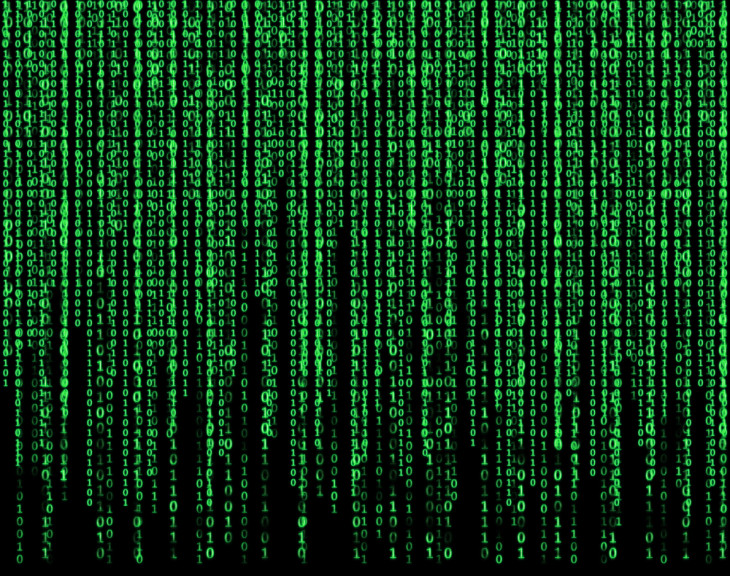
\includegraphics[width= 0.5\textwidth]{matrix.jpg}
  \caption{From movie ``The Matrix''}
  \label{fig:matrix}
\end{figure}
\end{frame}

\begin{frame}
{Definitions}
\begin{itemize}
 \item A matrix is a rectangular box of numbers,
 \begin{itemize}
 \item ex. 2 by 3 matrix 
 $$ A = 
\begin{bmatrix}
 2 & 1 & 15\\
 1 & 1 & 5\\
 \end{bmatrix}
$$
\end{itemize}
\item If a matrix has only one row or only one column it is called a vector, 
\begin{itemize}
 \item ex. 2 dimensional column vector 
 $$ b_{1} = 
\begin{bmatrix}
 15 \\
 5  \\
 \end{bmatrix}, 
 $$
\item ex. 2 dimensional  row vector
 $$  b_{2} = 
 \begin{bmatrix}
 15 &
 5  \\
 \end{bmatrix}, 
 $$
\end{itemize} 
\end{itemize}
\end{frame}

\section{Linear system (system of linear equation)}

\section{An  example in image processing}

 \begin{frame}%{Before and after a transformation}
\begin{columns}
    \begin{column}{0.5\textwidth}
        \begin{figure}
  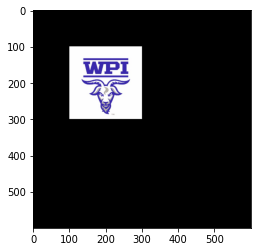
\includegraphics[width= 1\textwidth]{img1.png}
  \caption{Before  Transormation}
  \label{fig:goat1}
\end{figure}    \end{column}
    \begin{column}{0.5\textwidth}
        \begin{figure}
  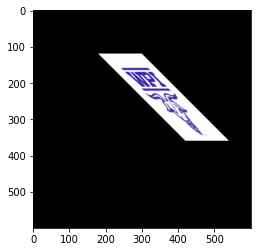
\includegraphics[width= 1\textwidth]{img2.png}
  \caption{After Transormation}
  \label{fig:goat2}
\end{figure}
    \end{column}
\end{columns}
\end{frame}

\begin{frame}
 %{Transformation as a mapping}
 
\begin{itemize}
 \item Transformation takes each coordinate vector to another coordinate vector by mapping
 $$ T:
\begin{bmatrix}
 x_{1}\\x_{2}
\end{bmatrix}
\mapsto 
\begin{bmatrix}
 \frac 1 2 x_{1} + x_{2}
 \\x_{2}
\end{bmatrix}
$$

\item (Q.) 
A corner of the new picture is
$\begin{bmatrix}
 350\\ 300
\end{bmatrix}$.
What is its original coordinate?
\end{itemize}
\end{frame}



 \begin{frame}%{As a linear system}
\begin{columns}
    \begin{column}{0.5\textwidth}
        
\begin{itemize}
 \item Set the original corner as 
 $\begin{bmatrix}
 x_{1}\\x_{2}
\end{bmatrix}$
\item Solve
\begin{equation*}
 \label{eq:01}
\left\{
\begin{array}
 {ll}
\frac 1 2 x_{1}  \ + & x_{2} = 350 \\
& x_{2} = 300
\end{array}
\right.
\end{equation*}
 \item The solution is ...
\end{itemize}   
\end{column}
    \begin{column}{0.5\textwidth}
   %text
    \end{column}
\end{columns}
\end{frame}
\section{General form of Linear System (System of Linear Equations)}
\begin{frame}
 %{General form }
\begin{columns}
\begin{column}
 {.7\textwidth}
 \begin{itemize}
 \item $m\times n$ linear system is 
\begin{equation*}
 \label{eq:02}
\left\{
\begin{array}
 {ll}
 a_{11} x_{1} + \cdots + a_{1n} x_{n} &= b_{1} \\
 a_{21} x_{1} + \cdots + a_{2n} x_{n} &= b_{2} \\
 \vdots \\
 a_{m1} x_{1} + \cdots + a_{mn} x_{n} &= b_{m}.
\end{array}
\right.
\end{equation*}
\item Coefficients $a_{ij}$ and $b_{i}$ are given numbers
\item The goal is to find the solution
$$x = 
\begin{bmatrix}
 x_{1}\\ x_{2}\\ \vdots\\ x_{m}
\end{bmatrix}
$$
\end{itemize}

\end{column}
\begin{column}
 {.3\textwidth}
% What is the solution of \eqref{eq:01}?
\end{column}
\end{columns}

 
\end{frame}



\begin{frame}
 %{Coefficient matrix and Augmented matrix}
\begin{columns}
\begin{column}
 {.7\textwidth}
 For $m\times n$ linear system,
 \begin{itemize}
 \item   coefficient matrix
$$ A = 
\begin{bmatrix}
 a_{11} & \cdots & a_{1n} \\
 a_{21} & \cdots & a_{2n} \\
 \vdots\\
 a_{m1} & \cdots & a_{mn} \\
\end{bmatrix}
$$
\item augmented matrix 
$[A\  |\  b ]$, i.e. 
$$\begin{bmatrix}
 a_{11} & \cdots & a_{1n} & | & b_{1} \\
 a_{21} & \cdots & a_{2n} & | & b_{2} \\
 \vdots\\
 a_{m1} & \cdots & a_{mn} & | & b_{m} \\
\end{bmatrix}
$$
\end{itemize}

\end{column}
\begin{column}
 {.3\textwidth}
% What is the solution of \eqref{eq:01}?
\end{column}
\end{columns}
\end{frame}

\section{Example}

\begin{frame}
 {}
\begin{columns}
\begin{column}
 {.4\textwidth}
Consider linear system
$$
\left\{
\begin{array}
 {ll}
  x_{1} \ + 2 x_{2} - x_{3} &= 4 \\
   - x_{1} - x_{2} +2 x_{3} &= 1 \\
  x_{1} \quad\quad\quad +  x_{3} &= 6 .
\end{array}
\right.
$$

 \begin{itemize}
 \item  write coefficient matrix
 \item write augmented matrix
 \item find its solution (next )
\end{itemize}

\end{column}
\begin{column}
 {.3\textwidth}
% What is the solution of \eqref{eq:01}?
\end{column}
\end{columns}
\end{frame}

\end{document}

